\documentclass[conference]{IEEEtran}
\usepackage{cite}
\usepackage{amsmath,amssymb,amsfonts}
\usepackage{graphicx}
\usepackage{textcomp}
\usepackage{xcolor}
\usepackage{url}
\usepackage{tikz}
\usetikzlibrary{shapes.geometric,arrows.meta,positioning,fit}
\usepackage{booktabs}
%\usepackage{multirow}

\begin{document}

\title{Safe and Efficient Robot Planning in Human Crowds}
\author{
\IEEEauthorblockN{Vaibhav Mehra \quad Muhammad Maaz \quad Benjamin Li}
\IEEEauthorblockA{
Department of Computer Science\\
University College London\\
London, United Kingdom\\
\{vaibhav.mehra.23, muhammad.maaz.23, benjamin.li.23\}@ucl.ac.uk}
}
\maketitle

% ─────────────────────────────────────────────────────────────────
\begin{abstract}
A robot moving through a crowd has to guess where each person will be
a few seconds from now, and how confident it can be in that guess.  Our
navigation stack pairs the predictor with a residual crowd-motion model
and synthetic data generator upstream, and a conformal safety layer
feeding a PPO-trained diffusion controller downstream; this report
covers the predictors.  We benchmark a Social-LSTM baseline, a
velocity-augmented variant (SLSTM+V), a bidirectional Social-GRU, a
Trajectory Transformer, and a diffusion predictor against CV and
Trajectron++ on ETH/UCY and SDD, then pretrain on SDD and fine-tune
jointly on ETH/UCY and our synthetic data.  Transformer wins on ETH/UCY
(ADE $0.568$\,m, NLL $1.54$, $12\times$ tighter than any recurrent
baseline); Trajectron++ alone covers multi-modal futures (minADE@20
$0.385$\,m).  SDD pretraining cuts recurrent ADE by $5$--$10\%$; the
Transformer barely moves.  Adding velocity to the focal input drops Social-LSTM's ADE on every
ETH/UCY and SDD scene we tested.
\end{abstract}

\begin{IEEEkeywords}
trajectory prediction, pedestrian motion, social LSTM, transformer,
diffusion models, transfer learning, crowd navigation
\end{IEEEkeywords}

% ─────────────────────────────────────────────────────────────────
\section{Introduction}
% TODO (joint): background, problem definition, overview of contributions.

% ─────────────────────────────────────────────────────────────────
\section{Project Management}
% TODO (joint): milestones, timeline, roles, risks.

% ─────────────────────────────────────────────────────────────────
\section{Methodology and System Design}

The predictor takes the output of the Residual Crowd Motion Model and
Synthetic Data Generator upstream and hands its forecasts to a
split-conformal safety layer plus a PPO-trained diffusion controller
downstream.  We describe the five predictor architectures in
Sec.~\ref{sec:tpm} and the transfer protocol that trains them in
Sec.~\ref{sec:transfer}.

% NOTE TO COLLABORATORS: Vaibhav's subsections
% (A. Synthetic Data Generation, B. Residual Crowd Motion Model)
% precede this content. The subsections below are Muhammad's contribution.

\subsection{Trajectory Prediction Models}
\label{sec:tpm}

Each predictor observes 8 steps at $2.5$\,Hz (3.2\,s) and emits 12
future steps (4.8\,s).  Coordinates are taken relative to the last
observed position, keeping models scene-agnostic
\cite{alahi2016social}.  Social context comes from up to five
neighbours inside a $2.0$\,m radius.  Outputs are a bivariate Gaussian
$(\mu_x, \mu_y, \sigma_x, \sigma_y, \rho)$ per future step, trained by
the per-step negative log-likelihood.

\subsubsection{Social-LSTM and Velocity-Augmented Variant}

Social-LSTM~\cite{alahi2016social} is an LSTM encoder--decoder
(hidden 128, embedding 64).  At each step it max-pools neighbour hidden
states inside $2.0$\,m and concatenates the result with the focal
position embedding before the LSTM update.  SLSTM+V keeps the same
architecture but appends the instantaneous velocity
$v_t = p_t - p_{t-1}$ to the focal input
($(x_t,y_t)\!\to\!(x_t,y_t,v_x,v_y)$).  Neighbour inputs stay 2-D.

\subsubsection{Bidirectional Social-GRU}

Social-GRU replaces the LSTM with a bidirectional
GRU~\cite{cho2014learning,schuster1997bidirectional}.  Forward and
backward hidden states ($2{\times}128$) are concatenated and projected
back to 128 before social pooling, so a late-window cue (say, a
pedestrian decelerating at step 6) can also reach earlier hidden
states.  Decoder and head are unchanged.

\subsubsection{Trajectory Transformer}

The Trajectory Transformer is a Pre-LN
encoder--decoder~\cite{vaswani2017attention,xiong2020layer} with
$d_\text{model}{=}128$, four attention heads, and two layers each
side.  Eight focal tokens go through self-attention; five neighbour
slots add $5\times 8 = 40$ tokens (masked per slot) for a 48-token
memory.  Twelve learned queries cross-attend to that memory, and a
shared linear head emits the bivariate Gaussian per step
(Fig.~\ref{fig:transformer}).

\begin{figure}[t]
  \centering
  \resizebox{0.6\columnwidth}{!}{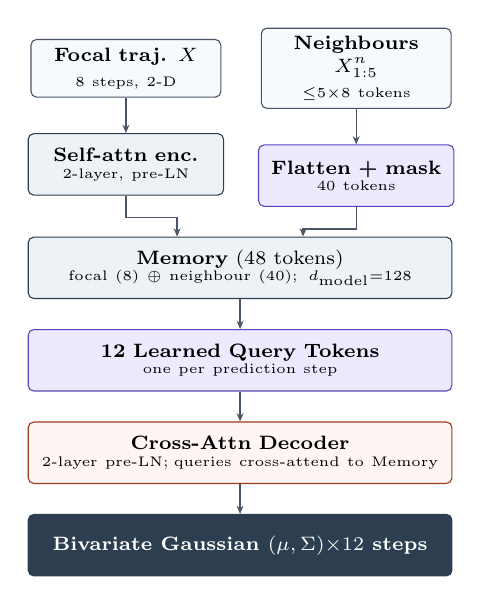
\begin{tikzpicture}[
  node distance=0.38cm,
  pGray/.style={rectangle, rounded corners=2pt,
    minimum width=2.4cm, minimum height=0.72cm,
    align=center, text width=2.2cm, inner sep=3pt,
    fill={rgb,255:red,247;green,250;blue,252},
    draw={rgb,255:red,74;green,85;blue,104},
    line width=0.4pt, font=\scriptsize},
  pTeal/.style={rectangle, rounded corners=2pt,
    minimum width=5.3cm, minimum height=0.78cm,
    align=center, text width=5.1cm, inner sep=4pt,
    fill={rgb,255:red,237;green,242;blue,247},
    draw={rgb,255:red,44;green,62;blue,80},
    line width=0.4pt, font=\scriptsize},
  pPurp/.style={rectangle, rounded corners=2pt,
    minimum width=5.3cm, minimum height=0.78cm,
    align=center, text width=5.1cm, inner sep=4pt,
    fill={rgb,255:red,237;green,233;blue,254},
    draw={rgb,255:red,83;green,74;blue,183},
    line width=0.4pt, font=\scriptsize},
  pCoral/.style={rectangle, rounded corners=2pt,
    minimum width=5.3cm, minimum height=0.78cm,
    align=center, text width=5.1cm, inner sep=4pt,
    fill={rgb,255:red,255;green,245;blue,245},
    draw={rgb,255:red,153;green,61;blue,30},
    line width=0.4pt, font=\scriptsize},
  pFinal/.style={rectangle, rounded corners=2pt,
    minimum width=5.3cm, minimum height=0.78cm,
    align=center, text width=5.1cm, inner sep=4pt,
    fill={rgb,255:red,44;green,62;blue,80},
    draw={rgb,255:red,44;green,62;blue,80},
    text=white, line width=0.4pt, font=\scriptsize\bfseries},
  parr/.style={-{Stealth[length=3pt,width=2.5pt]},
    line width=0.45pt,
    color={rgb,255:red,74;green,85;blue,104}},
]

  %% ── Input nodes ─────────────────────────────────────────────
  \node[pGray] (focal) {%
    {\bfseries Focal traj.} $X$\\[1pt]
    {\tiny 8 steps, 2-D}};
  \node[pGray, right=0.5cm of focal] (nbrs) {%
    {\bfseries Neighbours} $X^n_{1:5}$\\[1pt]
    {\tiny ${\leq}5{\times}8$ tokens}};

  %% ── Focal encoder (narrow, directly below focal) ────────────
  \node[pTeal, minimum width=2.4cm, text width=2.2cm,
    below=0.45cm of focal] (enc) {%
    {\bfseries Self-attn enc.}\\[-2pt]
    {\tiny 2-layer, pre-LN}};

  %% ── Neighbour flatten (narrow, directly below nbrs) ─────────
  \node[pPurp, minimum width=2.4cm, text width=2.2cm,
    below=0.45cm of nbrs] (flat) {%
    {\bfseries Flatten + mask}\\[-2pt]
    {\tiny 40 tokens}};

  %% ── Memory (full width, centred) ────────────────────────────
  \node[pTeal, below=0.52cm of enc, xshift=1.45cm] (mem) {%
    {\bfseries Memory} (48 tokens)\\[-2pt]
    {\tiny focal (8) $\oplus$ neighbour (40);\;\;$d_\text{model}{=}128$}};

  %% ── Learned queries ─────────────────────────────────────────
  \node[pPurp, below=0.38cm of mem] (qry) {%
    {\bfseries 12 Learned Query Tokens}\\[-2pt]
    {\tiny one per prediction step}};

  %% ── Cross-attention decoder ─────────────────────────────────
  \node[pCoral, below=0.38cm of qry] (dec) {%
    {\bfseries Cross-Attn Decoder}\\[-2pt]
    {\tiny 2-layer pre-LN;\;queries cross-attend to Memory}};

  %% ── Output ──────────────────────────────────────────────────
  \node[pFinal, below=0.38cm of dec] (out) {%
    Bivariate Gaussian $(\mu,\Sigma){\times}12$ steps};

  %% ── Arrows ───────────────────────────────────────────────────
  \draw[parr] (focal.south) -- (enc.north);
  \draw[parr] (nbrs.south)  -- (flat.north);

  \draw[parr] (enc.south)  -- ++(0,-0.28)
    -| ([xshift=-0.8cm]mem.north);
  \draw[parr] (flat.south) -- ++(0,-0.28)
    -| ([xshift=+0.8cm]mem.north);

  \foreach \f/\t in {mem/qry, qry/dec, dec/out}
    \draw[parr] (\f.south) -- (\t.north);

\end{tikzpicture}
}
  \caption{Trajectory Transformer architecture.}
  \label{fig:transformer}
\end{figure}

\subsubsection{Diffusion-Based Trajectory Predictor}

Denoising Diffusion Probabilistic Models~\cite{ho2020denoising}
reverse a Gaussian noise process to produce stochastic samples.  We
include one because the downstream shield consumes $K{=}20$ diverse
trajectories and diffusion supplies them without an explicit mixture.
A shared Transformer encoder produces a CLS summary and a full memory.
A Gaussian MLP reads the CLS token and emits the bivariate parameters
directly.  A separate denoiser $\varepsilon_\theta$ cross-attends to
the memory and predicts the noise term at each diffusion step.  We use $T{=}100$ steps with linear
$\beta \in [10^{-4}, 0.02]$, and a loss that sums the Gaussian-head NLL
with the DDPM MSE at weight $\lambda_\text{DDPM}{=}0.3$; larger weights
degraded point accuracy in sweeps.  In an early version we detached the Gaussian head's gradient from the
encoder.  Removing that detach, so that both heads update the shared
encoder together, cut ADE on ETH/UCY from $1.37$\,m to $0.58$\,m.
Sample diversity stayed roughly the same.  At
inference we draw $K=20$ samples with DDIM-50~\cite{song2021denoising}.

\subsection{Transfer Learning via SDD Pretraining}
\label{sec:transfer}

ETH/UCY's five scenes are too few to train recurrent models reliably
from scratch, so we adopt a two-stage protocol.  Stage one pretrains
each architecture on the Stanford Drone
Dataset~\cite{robicquet2016learning} (8 aerial scenes,
$\sim$249k sequences) leave-one-scene-out for up to 100 epochs at lr
$10^{-3}$.  Stage two fine-tunes each checkpoint at lr $10^{-4}$ for
up to 50 epochs (patience 15, grad-clip max-norm $1.0$) on a mixture
of the four ETH/UCY training scenes and the synthetic trajectories
from the residual crowd-motion model.  The three sources cover
different ground: SDD is broad but aerial and mixes cyclists with
pedestrians; ETH/UCY supplies real pedestrian behaviour on the same
ground as the test scene; the synthetic stream fills in the crowd
configurations the planner will face at deployment that neither real
dataset contains (Fig.~\ref{fig:finetune}).

\begin{figure}[t]
  \centering
  \resizebox{0.6\columnwidth}{!}{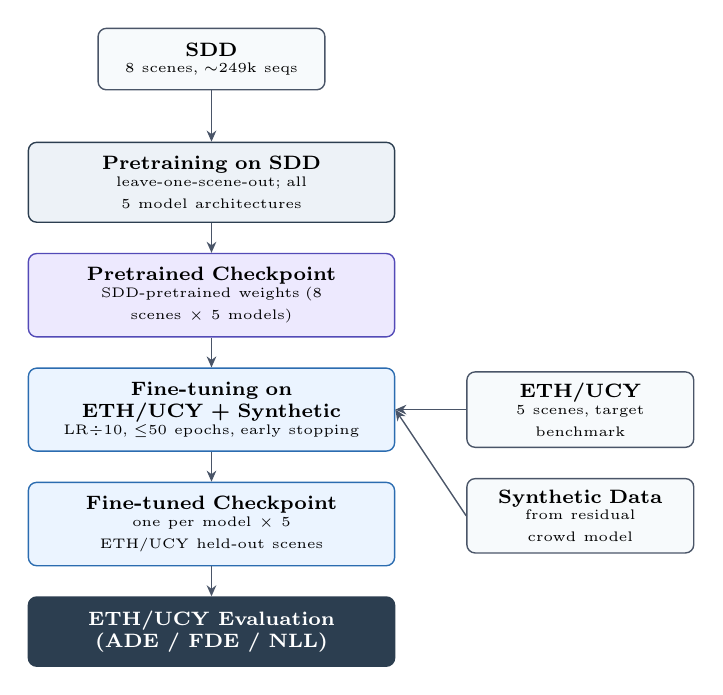
\begin{tikzpicture}[
  node distance=0.38cm,
  pinput/.style={rectangle, rounded corners=3pt,
    minimum width=2.8cm, minimum height=0.78cm,
    align=center, text width=2.6cm, inner sep=4pt,
    fill={rgb,255:red,247;green,250;blue,252},
    draw={rgb,255:red,74;green,85;blue,104},
    line width=0.5pt, font=\scriptsize},
  pTeal/.style={rectangle, rounded corners=3pt,
    minimum width=4.6cm, minimum height=0.85cm,
    align=center, text width=4.3cm, inner sep=5pt,
    fill={rgb,255:red,237;green,242;blue,247},
    draw={rgb,255:red,44;green,62;blue,80},
    line width=0.5pt, font=\scriptsize},
  pPurp/.style={rectangle, rounded corners=3pt,
    minimum width=4.6cm, minimum height=0.85cm,
    align=center, text width=4.3cm, inner sep=5pt,
    fill={rgb,255:red,237;green,233;blue,254},
    draw={rgb,255:red,83;green,74;blue,183},
    line width=0.5pt, font=\scriptsize},
  pAmb/.style={rectangle, rounded corners=3pt,
    minimum width=4.6cm, minimum height=0.85cm,
    align=center, text width=4.3cm, inner sep=5pt,
    fill={rgb,255:red,235;green,244;blue,255},
    draw={rgb,255:red,43;green,108;blue,176},
    line width=0.5pt, font=\scriptsize},
  pFinal/.style={rectangle, rounded corners=3pt,
    minimum width=4.6cm, minimum height=0.85cm,
    align=center, text width=4.3cm, inner sep=5pt,
    fill={rgb,255:red,44;green,62;blue,80},
    draw={rgb,255:red,44;green,62;blue,80},
    text=white, line width=0.5pt, font=\scriptsize\bfseries},
  parr/.style={-{Stealth[length=4pt,width=3.5pt]},
    line width=0.5pt,
    color={rgb,255:red,74;green,85;blue,104}},
]

  %% ── Pipeline nodes ──────────────────────────────────────────
  \node[pTeal] (pre) {%
    {\bfseries Pretraining on SDD}\\[-2pt]
    {\tiny leave-one-scene-out;\;all 5 model architectures}};
  \node[pPurp, below=0.38cm of pre] (ckpt) {%
    {\bfseries Pretrained Checkpoint}\\[-2pt]
    {\tiny SDD-pretrained weights\;(8 scenes ${\times}$ 5 models)}};
  \node[pAmb, below=0.38cm of ckpt] (ft) {%
    {\bfseries Fine-tuning on ETH/UCY + Synthetic}\\[-2pt]
    {\tiny LR${\div}10$,\;${\leq}50$ epochs,\;early stopping}};
  \node[pAmb, below=0.38cm of ft] (ftckpt) {%
    {\bfseries Fine-tuned Checkpoint}\\[-2pt]
    {\tiny one per model ${\times}$ 5 ETH/UCY held-out scenes}};
  \node[pFinal, below=0.38cm of ftckpt] (eval) {%
    ETH/UCY Evaluation (ADE / FDE / NLL)};

  %% ── Input nodes ─────────────────────────────────────────────
  \node[pinput, above=0.65cm of pre] (sdd) {%
    {\bfseries SDD}\\[-2pt]
    {\tiny 8 scenes,\;${\sim}249$k seqs}};
  \node[pinput, right=0.9cm of ft] (eth) {%
    {\bfseries ETH/UCY}\\[-2pt]
    {\tiny 5 scenes,\;target benchmark}};
  \node[pinput, below=0.38cm of eth] (synth) {%
    {\bfseries Synthetic Data}\\[-2pt]
    {\tiny from residual crowd model}};

  %% ── Arrows ──────────────────────────────────────────────────
  \draw[parr] (sdd.south)  -- (pre.north);
  \draw[parr] (eth.west)   -- (ft.east);
  \draw[parr] (synth.west) -- (ft.east);

  \foreach \f/\t in {pre/ckpt, ckpt/ft, ft/ftckpt, ftckpt/eval}
    \draw[parr] (\f.south) -- (\t.north);

\end{tikzpicture}
}
  \caption{Two-stage transfer: SDD pretrain $\Rightarrow$ joint
           ETH/UCY $+$ synthetic fine-tune.}
  \label{fig:finetune}
\end{figure}

% ─────────────────────────────────────────────────────────────────
\section{Experimental Setup}

We evaluate on ETH~\cite{pellegrini2009you} (eth, hotel) and
UCY~\cite{lerner2007crowds} (univ, zara1, zara2), the standard
five-scene benchmark at $2.5$\,Hz with 8 observation and 12 prediction
steps (3.2\,s / 4.8\,s), and on
SDD~\cite{robicquet2016learning} (8 campus scenes downsampled stride 12
to $2.5$\,Hz, pixels to metres at $0.0417$\,m/px, $\sim$249k pedestrian
sequences).  Both use leave-one-scene-out cross-validation with results
averaged over held-out scenes.  We report ADE and FDE (mean and final
$\ell_2$ error in metres, $\downarrow$), minADE@20 and minFDE@20 (best
of $K{=}20$ samples, $\downarrow$), and NLL (bivariate Gaussian,
$\downarrow$; undefined for CV).  Baselines are constant-velocity (CV)
extrapolation with Gaussian noise and
Trajectron++~\cite{salzmann2020trajectron} (graph-based CVAE, trained
100 epochs per held-out scene).  All learned models use Adam
(lr $10^{-3}$, weight decay $10^{-4}$, batch 64) with a
\texttt{ReduceLROnPlateau} scheduler (patience 5, factor 0.5).  Scratch
ETH/UCY trains up to 200 epochs (patience 20); SDD pretraining up to
100 epochs; fine-tuning at lr $10^{-4}$ up to 50 epochs (patience 15,
grad-clip max-norm 1.0).

% ─────────────────────────────────────────────────────────────────
\section{Results and Discussion}

Transformer takes the lowest ADE in Table~\ref{tab:ethucy} at
$0.568$\,m, with NLL $1.54$.  That NLL is more than ten times tighter
than the next recurrent model.  Only Trajectron++ produces samples
that meaningfully spread across futures: its minADE@20 of $0.385$\,m
beats every other entry by at least $0.20$\,m.  Pretraining on SDD and
then fine-tuning on ETH/UCY plus our synthetic data cuts recurrent
ADE by $5$ to $10$ per cent (Table~\ref{tab:finetune}).  The
Transformer barely moves.

Because the encoder is non-causal, the variance head reads the entire
8-step window at every position.  A late-window cue such as a
pedestrian starting to decelerate at step 6 therefore informs the
sigma estimate at every earlier step, whereas a causal LSTM has only
seen up to step 6 by that point.  A tighter sigma feeds directly into
a smaller conformal radius.

\begin{table}[t]
\caption{ETH/UCY leave-one-out results averaged over 5 scenes.
         Best value per metric in \textbf{bold}. mADE/mFDE = minADE@20 / minFDE@20.}
\label{tab:ethucy}
\centering
\footnotesize
\setlength{\tabcolsep}{4pt}
\begin{tabular}{@{}lrrrrr@{}}
\toprule
Model
  & ADE$\downarrow$
  & FDE$\downarrow$
  & mADE@20$\downarrow$
  & mFDE@20$\downarrow$
  & NLL$\downarrow$ \\
\midrule
CV Baseline
  & 0.736 & 1.272 & 0.610 & 0.814 & --- \\
Social-LSTM~\cite{alahi2016social}
  & 0.596 & 1.248 & 0.581 & 0.597 & 18.0 \\
SLSTM+V (ours)
  & 0.585 & 1.240 & 0.587 & 0.585 & 36.2 \\
Social-GRU (ours)
  & 0.586 & 1.238 & 0.596 & 0.924 & --- \\
Transformer (ours)
  & \textbf{0.568} & 1.203 & 0.638 & \textbf{0.532} & \textbf{1.54} \\
Diffusion (ours)
  & 0.579 & \textbf{1.195} & 1.174 & 2.032 & 5.14 \\
Trajectron++~\cite{salzmann2020trajectron}
  & 0.853 & 1.817 & \textbf{0.385} & 0.674 & 8.49 \\
\bottomrule
\end{tabular}
\end{table}

Sharper means come at the cost of weaker diversity.  Split-conformal
calibration measures predictor residuals on a held-out set and takes
the $(1-\alpha)$ quantile as the safety radius, so that radius scales
with the predictor's mean error.  A tight Transformer therefore yields
a smaller radius than the wider, mean-biased Trajectron++; we pair the
Transformer's mean prediction with a conformal radius calibrated on its
own residuals, which gave the smallest safety radius of any pairing we
tested.

Velocity augmentation lowers ADE on every scene: $0.596$\,m for
Social-LSTM down to $0.585$\,m for SLSTM+V (a $1.8\%$ relative drop for
two extra input channels), largest on univ and zara1 (frequent
direction changes), smallest on zara2 (uniform sidewalk motion).
Social-GRU matches Social-LSTM almost exactly on ADE ($0.586$ vs
$0.596$\,m) with a slim FDE edge ($1.238$ vs $1.248$\,m); the encoder
is not the binding constraint, social pooling probably is.  Performance
varies sharply by scene: eth is hardest (all models in
$0.98$--$1.03$\,m), zara2 easiest ($0.32$--$0.37$\,m), and eth also
gains least from SDD fine-tuning (Social-LSTM $-5.9\%$ on eth vs
$-29.8\%$ on hotel), suggesting eth lies outside the convex hull of both
SDD and the synthetic stream; the shield's calibration set should
weight scenes by deployment similarity.  The Diffusion model takes the
lowest FDE ($1.195$\,m) yet a high minADE@20 ($1.174$\,m): its $K=20$
samples cluster tightly around the mean because the 49-token memory
already pins down the trajectory and DDIM-50 leaves little entropy
before the conditioning dominates.  Note this is our offline diffusion predictor, not the PPO-trained
diffusion policy used inside the safety layer.

\begin{figure}[t]
  \centering
  \includegraphics[width=0.88\columnwidth]{figures/fig03_qualitative.png}
  \caption{Qualitative prediction on four zara1 scenarios.  Both models
           track the dominant direction in Scenarios 1--3 and diverge
           on Scenario 4's sharp turn.  Per-panel ADEs are close;
           Social-LSTM happens to win three of these four random samples
           even though the Transformer leads on the dataset average
           (Table~\ref{tab:ethucy}).}
  \label{fig:qualitative}
\end{figure}

On SDD (Table~\ref{tab:sdd}), every learned model cuts CV ADE by
$27$--$30\%$.  SLSTM+V wins on ADE ($0.656$\,m), minADE@20, and
minFDE@20; the Transformer wins on FDE ($1.326$\,m); velocity helps
more here than on ETH/UCY because cyclists and turning manoeuvres make
it useful as a separate channel.  Diffusion's minADE@20 stays high
($1.710$\,m), the same collapse seen on ETH/UCY.

\begin{table}[t]
\caption{SDD leave-one-out results averaged over 8 scenes.
         Best value per metric in \textbf{bold}.}
\label{tab:sdd}
\centering
\footnotesize
\setlength{\tabcolsep}{4pt}
\begin{tabular}{@{}lrrrrr@{}}
\toprule
Model
  & ADE$\downarrow$
  & FDE$\downarrow$
  & mADE@20$\downarrow$
  & mFDE@20$\downarrow$
  & NLL$\downarrow$ \\
\midrule
CV Baseline
  & 0.926 & 1.620 & 0.797 & 1.154 & --- \\
Social-LSTM
  & 0.672 & 1.358 & 0.783 & 0.621 & \textbf{1.162} \\
SLSTM+V (ours)
  & \textbf{0.656} & 1.340 & \textbf{0.755} & \textbf{0.604} & 1.289 \\
Social-GRU (ours)
  & 0.667 & 1.379 & 0.793 & 0.625 & 1.331 \\
Transformer (ours)
  & 0.657 & \textbf{1.326} & 0.808 & 0.633 & 1.474 \\
Diffusion (ours)
  & 0.673 & 1.335 & 1.710 & 3.159 & 1.683 \\
\bottomrule
\end{tabular}
\end{table}

Table~\ref{tab:finetune} compares scratch ETH/UCY against the same
models pretrained on SDD and fine-tuned jointly on ETH/UCY and
synthetic data.  All recurrent models improve: Social-LSTM by $9.9\%$
($0.596 \to 0.537$\,m), Social-GRU by $6.3\%$, SLSTM+V by $5.1\%$.  The
Transformer barely moves ($+0.4\%$): with $\sim$5k training sequences
per held-out scene the 537k-parameter Transformer is already
over-parameterised for ETH/UCY; SDD adds quantity but not a new
distribution to exploit.

\begin{table}[t]
\caption{SDD pretraining then ETH/UCY+synthetic fine-tuning, ETH/UCY
         ADE (m, avg.\ over 5 scenes).  $\Delta$ vs.\ scratch.}
\label{tab:finetune}
\centering
\footnotesize
\setlength{\tabcolsep}{4pt}
\begin{tabular}{@{}lrrr@{}}
\toprule
Model & Scratch & SDD then Synth FT & $\Delta$ (\%) \\
\midrule
Social-LSTM  & 0.596 & \textbf{0.537} & $-9.9$ \\
SLSTM+V      & 0.585 & 0.555          & $-5.1$ \\
Social-GRU       & 0.586 & 0.549          & $-6.3$ \\
Transformer  & \textbf{0.568} & 0.570 & $+0.4$ \\
Diffusion    & 0.579 & 0.535          & $-7.6$ \\
\bottomrule
\end{tabular}
\end{table}

For the recurrent models, SDD effectively acts as a regulariser;
fine-tuning then narrows the predictor onto the target distribution.
The Transformer already saturates the information in ETH/UCY's
interaction patterns, so adding broadly similar data brings no
additional gain~\cite{kornblith2019better}.  Diffusion's minADE@20
also fails to improve after fine-tuning, moving only from $1.174$\,m
to $1.157$\,m, which confirms its diversity ceiling is architectural,
not distributional.

A few caveats are worth flagging.  ETH/UCY's five scenes at $2.5$\,Hz
are a narrow basis for any general claim about the accuracy--diversity
tradeoff.  All five models share a $2.0$\,m social-pooling radius, so
the Social-GRU versus Social-LSTM near-tie may partly reflect that
shared parameter rather than the encoder difference alone.  Our
Trajectron++ baseline ran only 100 epochs per held-out scene, shorter
than the published schedule.  And the scene-asymmetric transfer benefit
(most visibly on eth) suggests calibration-set design matters as much as
pretraining scale.

% ─────────────────────────────────────────────────────────────────
\section{Conclusions}
% TODO (joint): summary, challenges, insights, limitations, lessons.

\bibliographystyle{ieeetr}
\bibliography{references}

\end{document}
